\documentclass[standalone, version=2.0]{huangfusl-template}
\begin{document}
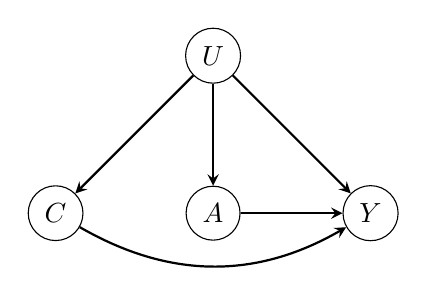
\begin{tikzpicture}
    \node[circle, draw] (C) at (-3, -1) {$C$};
    \node[circle, draw] (U) at (-1, 1) {$U$};
    \node[circle, draw] (A) at (-1, -1) {$A$};
    \node[circle, draw] (Y) at (1, -1) {$Y$};

    \draw[-stealth, thick] (C) to[bend right=30] (Y);
    \draw[-stealth, thick] (U) -- (A);
    \draw[-stealth, thick] (U) -- (Y);
    \draw[-stealth, thick] (A) -- (Y);
    \draw[-stealth, thick] (U) -- (C);
\end{tikzpicture}
\end{document}